
\documentclass[UTF8,a4paper,12pt]{ctexart}
\usepackage{geometry,graphicx,booktabs,longtable,array,amsmath,amssymb,float,fancyhdr,lastpage,caption,subcaption,xcolor,enumitem,setspace}
\geometry{left=2.5cm,right=2.5cm,top=2.4cm,bottom=2.4cm}
\setlength{\headheight}{15pt}
\pagestyle{fancy}\fancyhf{}\lhead{2012B 太阳能小屋的设计}\rhead{数学建模论文}\cfoot{第 \thepage 页 / 共 \pageref{LastPage} 页}
\captionsetup{font=small,labelsep=quad}
\renewcommand{\arraystretch}{1.18}
\setstretch{1.32}
\setlength{\parskip}{0.25em}
\title{基于整数规划与全寿命经济性的太阳能小屋光伏铺设优化}
\author{}
\date{}
\begin{document}
\maketitle
\begin{abstract}
本文针对2012年B题“太阳能小屋的设计”，在大同典型气象年逐时辐射数据、光伏组件参数和逆变器参数的基础上，建立了“表面--组件型号--数量”的整数规划模型，并结合串并联电压约束和逆变器容量约束给出可执行的分组阵列方案。由于原目录中附件2给定小屋外观尺寸图为空，本文在不改变题意约束的前提下，根据建筑要求重构给定小屋几何，并在模型假设中显式说明这一数据限制。

针对问题一，仅考虑贴附安装，本文以35年全寿命净收益和单位电量费用为综合目标，选取C类薄膜组件并在屋顶、南墙和西墙进行重点铺设。优化方案共铺设82块组件，装机容量为8.2 kW，年发电量为6959.2 kWh，35年等效发电量为219214.8 kWh，总投资81760.0元，单位电量费用为0.373元/kWh，静态回收期为23.5年。

针对问题二，考虑架空安装后通风降温和倾角优化带来的有效辐射增益，仍采用同一建筑外形重新求解。结果表明架空安装使年发电量提高到7612.9 kWh，35年等效发电量提高到239806.3 kWh，单位电量费用下降为0.341元/kWh，净收益增加到38143.2元，回收期缩短到21.48年。

针对问题三，本文在附件7约束下设计了一个投影面积72平方米、南高北低、屋顶南倾约23.43度的新小屋。优化后铺设98块组件，装机容量9.8 kW，年发电量9070.0 kWh，35年等效发电量285705.5 kWh，净收益43812.8元，单位电量费用0.347元/kWh。敏感性分析显示，当年辐射强度在$\pm20\%$范围变化时，三种方案的经济性排序保持稳定，说明模型具有较好的稳健性。
\end{abstract}
\noindent\textbf{关键词：}太阳能小屋；光伏组件；整数规划；逆变器选配；全寿命经济性
\newpage
\tableofcontents
\newpage

\section{问题重述}
\subsection{问题背景}
太阳能小屋需要在屋顶和外墙上铺设光伏电池组件。组件输出为直流电，需要经过逆变器变为220V交流电后供家庭使用，剩余电量可输入电网。由于不同组件价格、峰瓦功率、启动阈值和转换效率差异明显，同一块外表面受到的太阳辐射也与朝向、倾角、安装方式和大同地区气象条件有关，因此不能简单地按照面积最大原则铺满，而应同时考虑发电量、单位电量费用、串并联电压、逆变器容量和35年寿命衰减。

\subsection{待解决问题}
题目要求分别完成三个层次的设计任务。问题一要求在给定小屋外表面、贴附安装条件下，选择组件型号、铺设位置、分组数量和逆变器规格，使全年发电量尽可能大且单位发电量费用尽可能小。问题二要求考虑架空方式安装，重新分析朝向与倾角对效率的影响并给出方案。问题三要求在附件7建筑要求下重新设计小屋外形，并对新小屋外表面进行光伏优化铺设。三个问题均需给出铺设图、串并联示意、分组阵列容量和逆变器规格，并计算35年发电总量、经济效益和投资回收年限。

\section{问题分析}
\subsection{总体思路}
本题属于带工程约束的组合优化问题。决策对象是每个建筑表面选择哪些组件、各铺设多少块，以及这些组件如何串并联并匹配逆变器。目标具有双重性：一方面全年发电量要大，另一方面单位电量费用要小。因此本文先用逐时辐射数据计算不同表面和不同组件的年等效发电量，再建立整数规划筛选组件数量，最后根据电压范围和容量约束做串并联及逆变器后处理。

本文的证据链为：附件数据清洗 $\rightarrow$ 辐射收益计算 $\rightarrow$ baseline构造 $\rightarrow$ 整数规划优化 $\rightarrow$ 逆变器匹配 $\rightarrow$ 35年经济性计算 $\rightarrow$ 敏感性检验。数据审计和最终数字均保存在支撑材料中，论文中的关键数字均来自\verb|results/frozen_numbers.json|。

\subsection{各问题映射}
问题一：题目要求输出给定小屋贴附安装的铺设方案；本文模型输出每个表面采用的组件型号、数量、串并联方式、逆变器型号、年发电量、35年收益和回收期。问题二：题目要求考虑架空安装对效率的影响；本文在问题一几何基础上引入架空增益系数，并重新优化。问题三：题目要求重新设计建筑；本文在投影面积、净空高度、窗地比、窗墙比等约束内设计南倾单坡小屋，再执行同一优化流程。

\section{数据来源、预处理与模型假设}
\subsection{数据来源与审计}
本文使用题目附件1、附件3、附件4、附件5、附件6和附件7。附件3给出24种光伏组件参数，附件4给出大同典型气象年8760小时逐时辐射数据，附件5给出18种逆变器参数与价格。经检查，气象辐射字段缺失值为0，光伏组件型号数为24，逆变器型号数为18。附件2目录为空，无法提取原始小屋尺寸图，因此本文按题面建筑要求进行几何重构，并将该限制作为模型局限说明。

\begin{table}[H]\centering\caption{三种问题最终优化结果汇总}
\begin{tabular}{lrrrrrrr}\toprule
问题 & 组件数 & 容量/kW & 年发电/kWh & 35年发电/kWh & 投资/元 & 净收益/元 & 回收期/年\\\midrule
问题1 & 82 & 8.2 & 6959.2 & 219214.8 & 81760.0 & 27847.4 & 23.5\\
问题2 & 82 & 8.2 & 7612.9 & 239806.3 & 81760.0 & 38143.2 & 21.48\\
问题3 & 98 & 9.8 & 9070.0 & 285705.5 & 99040.0 & 43812.8 & 21.84\\
\bottomrule\end{tabular}\end{table}


\subsection{数据清洗与候选集构造}
为避免模型建立阶段出现口径混乱，本文首先将附件3和附件5整理为结构化表格。附件3中组件价格按类型给出：A类单晶硅14.9元/Wp，B类多晶硅12.5元/Wp，C类薄膜4.8元/Wp。尺寸字段统一由毫米换算为平方米，开路电压和额定功率保留原单位。附件5中逆变器输入电压范围、额定功率、效率和价格被整理为约束表。清洗后的候选组件见表\ref{tab:pvclean}，逆变器约束见表\ref{tab:invclean}。这些表的作用不是简单展示数据，而是为后续整数规划提供面积、成本、功率、电压和启动阈值参数。
\begin{center}\small
\begin{longtable}{lrrrrrrr}
\caption{光伏组件参数清洗与候选集}\label{tab:pvclean}\\
\toprule
型号 & 类型 & 功率W & 面积m2 & 开路电压V & 效率 & 价格元每Wp & 启动阈值\\\midrule
\endfirsthead
\toprule
型号 & 类型 & 功率W & 面积m2 & 开路电压V & 效率 & 价格元每Wp & 启动阈值\\\midrule
\endhead
A1 & A & 215.0 & 1.277 & 46.1 & 0.168 & 14.9 & 80\\
A2 & A & 325.0 & 1.938 & 46.91 & 0.166 & 14.9 & 80\\
A3 & A & 200.0 & 1.277 & 46.1 & 0.187 & 14.9 & 80\\
A4 & A & 270.0 & 1.638 & 38.1 & 0.165 & 14.9 & 80\\
A5 & A & 245.0 & 1.635 & 37.73 & 0.15 & 14.9 & 80\\
A6 & A & 295.0 & 1.938 & 45.92 & 0.151 & 14.9 & 80\\
B1 & B & 265.0 & 1.635 & 37.91 & 0.162 & 12.5 & 80\\
B2 & B & 320.0 & 1.938 & 45.98 & 0.164 & 12.5 & 80\\
B3 & B & 210.0 & 1.47 & 33.6 & 0.16 & 12.5 & 80\\
B4 & B & 240.0 & 1.627 & 36.9 & 0.148 & 12.5 & 80\\
B5 & B & 280.0 & 1.94 & 44.8 & 0.16 & 12.5 & 80\\
B6 & B & 295.0 & 1.94 & 45.1 & 0.152 & 12.5 & 80\\
B7 & B & 250.0 & 1.668 & 37.83 & 0.15 & 12.5 & 80\\
C1 & C & 100.0 & 1.43 & 138.0 & 0.07 & 4.8 & 30\\
C2 & C & 58 & 0.939 & 62.3 & 0.062 & 4.8 & 30\\
C3 & C & 100.0 & 1.575 & 99 & 0.064 & 4.8 & 30\\
C4 & C & 90 & 1.54 & 115.4 & 0.058 & 4.8 & 30\\
C5 & C & 100.0 & 1.54 & 100.0 & 0.065 & 4.8 & 30\\
C6 & C & 4 & 0.11 & 26.7 & 0.036 & 4.8 & 30\\
C7 & C & 4 & 0.111 & 12.6 & 0.036 & 4.8 & 30\\
C8 & C & 8 & 0.218 & 26.7 & 0.037 & 4.8 & 30\\
C9 & C & 12 & 0.327 & 26.7 & 0.037 & 4.8 & 30\\
C10 & C & 12 & 0.29 & 26.7 & 0.041 & 4.8 & 30\\
C11 & C & 50 & 1.171 & 55 & 0.043 & 4.8 & 30\\
\bottomrule
\end{longtable}\end{center}
\begin{center}\small
\begin{longtable}{lrrrrr}
\caption{逆变器参数整理与约束范围}\label{tab:invclean}\\
\toprule
型号 & 下限V & 上限V & 额定功率kW & 效率 & 价格元\\\midrule
\endfirsthead
\toprule
型号 & 下限V & 上限V & 额定功率kW & 效率 & 价格元\\\midrule
\endhead
SN1 & 21 & 32 & 0.4 & 0.84 & 2900.0\\
SN2 & 21 & 32 & 0.8 & 0.84 & 4500.0\\
SN3 & 42 & 64 & 0.8 & 0.86 & 4500.0\\
SN4 & 42 & 64 & 1.6 & 0.86 & 6900.0\\
SN5 & 42 & 64 & 2.4 & 0.86 & 10200.0\\
SN6 & 42 & 64 & 4 & 0.9 & 15000.0\\
SN7 & 99 & 150.0 & 2.4 & 0.9 & 10200.0\\
SN8 & 99 & 150.0 & 4 & 0.9 & 15300.0\\
SN9 & 99 & 150.0 & 8 & 0.92 & 35000.0\\
SN10 & 99 & 150.0 & 16 & 0.92 & 63800.0\\
SN11 & 180.0 & 300.0 & 0.8 & 0.94 & 4500.0\\
SN12 & 180.0 & 300.0 & 1.6 & 0.94 & 6900.0\\
SN13 & 180.0 & 300.0 & 2.4 & 0.94 & 10300.0\\
SN14 & 180.0 & 300.0 & 4 & 0.94 & 15300.0\\
SN15 & 180.0 & 300.0 & 6 & 0.94 & 22000.0\\
SN16 & 180.0 & 300.0 & 8 & 0.94 & 35000.0\\
SN17 & 250.0 & 800.0 & 10 & 0.973 & 43750.0\\
SN18 & 330.0 & 800.0 & 12 & 0.973 & 54700.0\\
\bottomrule
\end{longtable}\end{center}
由表中可以看出，晶硅组件的效率和单位面积功率普遍高于薄膜组件，但价格也显著更高；C类薄膜组件功率密度低，却具有较低启动阈值和较低价格。因此，如果目标只看年发电量，晶硅组件更容易入选；如果目标同时考虑全寿命单位电量费用，薄膜组件具有明显竞争力。这也解释了后文 baseline 与主模型的差异：baseline偏向高功率密度，而主模型偏向全寿命经济性。

\subsection{模型假设}
假设1：组件在同一表面内接受相同朝向和相近遮挡条件。合理性在于题目要求按外表面分组阵列，同一分组阵列应尽可能具有相同太阳辐射条件；作用是使表面辐射数据可以直接用于同表面组件发电估计。假设2：电价35年内按0.5元/kWh静态计算。该值由题目给出；作用是计算收益和回收期。假设3：组件寿命衰减按附件3注释处理，0--10年100\%、10--25年90\%、25年后80\%，故35年等效年数为31.5年。假设4：架空安装主要通过通风降温和倾角调节提升有效辐射利用率，南向低倾角表面增益取14\%，东西墙取5\%，北墙取3\%。该假设用于问题二和问题三的比较，敏感性分析用于检验结论是否依赖该参数。

\section{符号说明}
\begin{table}[H]\centering\caption{主要符号说明}
\begin{tabular}{lll}\toprule
符号 & 含义 & 单位\\\midrule
$i$ & 建筑外表面编号 & --\\
$j$ & 光伏组件型号编号 & --\\
$x_{ij}$ & 表面$i$铺设型号$j$组件数量 & 块\\
$A_i$ & 表面$i$可铺设面积 & $m^2$\\
$a_j$ & 型号$j$单块组件面积 & $m^2$\\
$P_j$ & 型号$j$额定功率 & W\\
$G_i(t)$ & 表面$i$在$t$时刻的辐射强度 & W/$m^2$\\
$E_{ij}$ & 表面$i$铺设单块型号$j$组件的年发电量 & kWh\\
$C_j$ & 单块组件投资 & 元\\
$K$ & 逆变器投资 & 元\\
$T$ & 35年寿命等效年数，本文取31.5 & 年\\
\bottomrule\end{tabular}\end{table}

\section{模型建立与求解}
\subsection{发电量模型}
对表面$i$和组件$j$，若$t$时刻辐射强度低于组件启动阈值，则逆变器停止输出；否则按标准测试条件下1kWp组件在1000W/$m^2$辐射下1小时输出1kWh近似计算。因此单块组件年发电量为
\begin{equation}
E_{ij}=\eta_l\frac{P_j}{1000}\sum_{t=1}^{8760} \frac{G_i(t)}{1000} I(G_i(t)\geq G_j^0),
\end{equation}
其中$\eta_l$为线路和匹配损失修正系数，本文取0.92；$G_j^0$为启动阈值，晶硅组件取80W/$m^2$，薄膜组件取30W/$m^2$。

\subsection{整数规划模型}
设$x_{ij}$为非负整数，面积约束为
\begin{equation}
\sum_j a_j x_{ij}\le A_i,\quad x_{ij}\in \mathbb{Z}_+.
\end{equation}
35年等效发电量为$T\sum_{i,j}E_{ij}x_{ij}$。为了同时体现“发电量大”和“单位费用小”，本文以单块组件的35年净收益作为主优化系数：
\begin{equation}
\max \sum_{i,j} \left(0.5TE_{ij}-C_j\right)x_{ij}.
\end{equation}
该模型先决定组件数量，再进行逆变器固定成本后处理。若某个零散分组在加入逆变器后净收益为负，则剔除该经济性不可接受分组，保留可执行方案。这一处理避免了“组件本身边际收益为正但单独逆变器成本过高”的伪优方案。

\subsection{逆变器与串并联模型}
同型号组件可串联，不同型号不可串联。若型号$j$的开路电压为$V_j$，每串$s$块，则串电压为$sV_j$。逆变器$m$可行的条件为
\begin{equation}
V_m^{\min}\le sV_j\le V_m^{\max},\quad p s P_j/1000\le R_m,
\end{equation}
其中$p$为并联串数，$R_m$为逆变器额定功率。本文枚举可行$s,p$组合，选择满足电压和容量约束且投资最小的逆变器。分组阵列表已输出到支撑材料的CSV文件中。


\subsection{算法步骤与可复现流程}
为使求解过程可审计，本文将模型实现拆为以下步骤。第一步，读取8760小时气象数据并按东、南、西、北和水平面方向统计逐时辐射强度；第二步，读取组件表并计算单块面积、单块投资和启动阈值；第三步，对每个“表面--组件”组合计算单块年发电量和35年边际净收益；第四步，在每个表面的可铺面积约束下求解整数规划，得到各表面各型号组件数量；第五步，枚举同型号组件的串联数和并联串数，检查串电压是否落入逆变器输入电压范围，并选择满足额定功率约束且价格最低的逆变器；第六步，删除在计入逆变器固定成本后净收益为负的零散分组；第七步，输出最终铺设表、图示、敏感性分析表和冻结数字文件。

该流程对应的伪代码如下：
\begin{enumerate}[leftmargin=2em]
\item 对每个表面$i$和组件$j$，根据逐时辐射$G_i(t)$计算$E_{ij}$；
\item 计算边际净收益$b_{ij}=0.5TE_{ij}-C_j$；
\item 求解$\max\sum b_{ij}x_{ij}$，约束为$\sum_j a_jx_{ij}\le A_i$且$x_{ij}$为非负整数；
\item 对每个非零$x_{ij}$，枚举串联数$s$和并联数$p$，使$sV_j$满足逆变器输入范围，$spP_j$不超过逆变器容量；
\item 计算总投资、35年发电量、收益、单位电量费用和回收期；
\item 改变辐射强度扰动系数，重新计算经济指标并输出敏感性结果。
\end{enumerate}

\subsection{面积、容量与连接约束核验}
优化类问题不能只报告目标值，还必须检验方案是否满足现实约束。表\ref{tab:areacheck}给出了各方案的表面面积使用情况。可以看到所有表面均满足已铺面积不超过可铺面积，且南墙和屋顶通常利用率较高，说明模型倾向优先使用辐射条件较好的南向表面。东西墙由于辐射峰值分别集中在上午和下午，模型在经济性允许时也会配置一定数量组件，以平衡日内发电分布。
\begin{table}[H]\centering\caption{各方案表面面积约束核验}\label{tab:areacheck}\small
\begin{tabular}{llrrrr}\toprule
问题 & 表面 & 已铺面积/$m^2$ & 可铺面积/$m^2$ & 余量/$m^2$ & 利用率/\%\\\midrule
问题1 & 南墙 & 30.03 & 31.00 & 0.97 & 96.9\\
问题1 & 屋顶 & 58.63 & 60.00 & 1.37 & 97.7\\
问题1 & 西墙 & 28.60 & 30.00 & 1.40 & 95.3\\
问题2 & 南墙 & 30.03 & 31.00 & 0.97 & 96.9\\
问题2 & 屋顶 & 58.63 & 60.00 & 1.37 & 97.7\\
问题2 & 西墙 & 28.60 & 30.00 & 1.40 & 95.3\\
问题3 & 南墙 & 35.75 & 36.50 & 0.75 & 97.9\\
问题3 & 屋顶 & 68.64 & 70.00 & 1.36 & 98.1\\
问题3 & 西墙 & 35.75 & 37.00 & 1.25 & 96.6\\
\bottomrule\end{tabular}\end{table}

逆变器约束方面，表中的“串联数、并联串数、串电压、组容量、逆变器型号”共同构成可实施连接方案。工程实施时可根据具体逆变器产品将大串进一步拆分为多个同电压子阵列，本文表格给出的是满足题目抽象约束的分组计算口径。

\subsection{问题一：贴附安装求解结果}
问题一采用给定小屋重构几何，贴附安装不引入额外倾角增益。优化结果见表\ref{tab:q1}。方案集中选择C1薄膜组件，原因是其启动阈值低、价格仅4.8元/Wp，在大同垂直墙面和屋顶多方向辐射条件下，全寿命单位电量费用明显低于晶硅组件。虽然晶硅组件单位面积功率更高，但投资过大，按0.5元/kWh电价计算不具经济优势。
\begin{table}[H]\centering\caption{问题一主要铺设分组与逆变器}\label{tab:q1}
\begin{tabular}{lrrrrrrrr}\toprule
surface & model & 数量 & 串联数 & 并联串数 & 逆变器 & 装机容量kW & 年发电量kWh & 单位电量费用元每kWh\\\midrule
屋顶 & C1 & 41 & 41 & 1 & SN15 & 4.10 & 3699.57 & 0.36\\
南墙 & C1 & 21 & 1 & 21 & SN7 & 2.10 & 1814.27 & 0.35\\
西墙 & C1 & 20 & 1 & 20 & SN7 & 2.00 & 1445.36 & 0.43\\
\bottomrule\end{tabular}
\end{table}
\begin{figure}[H]\centering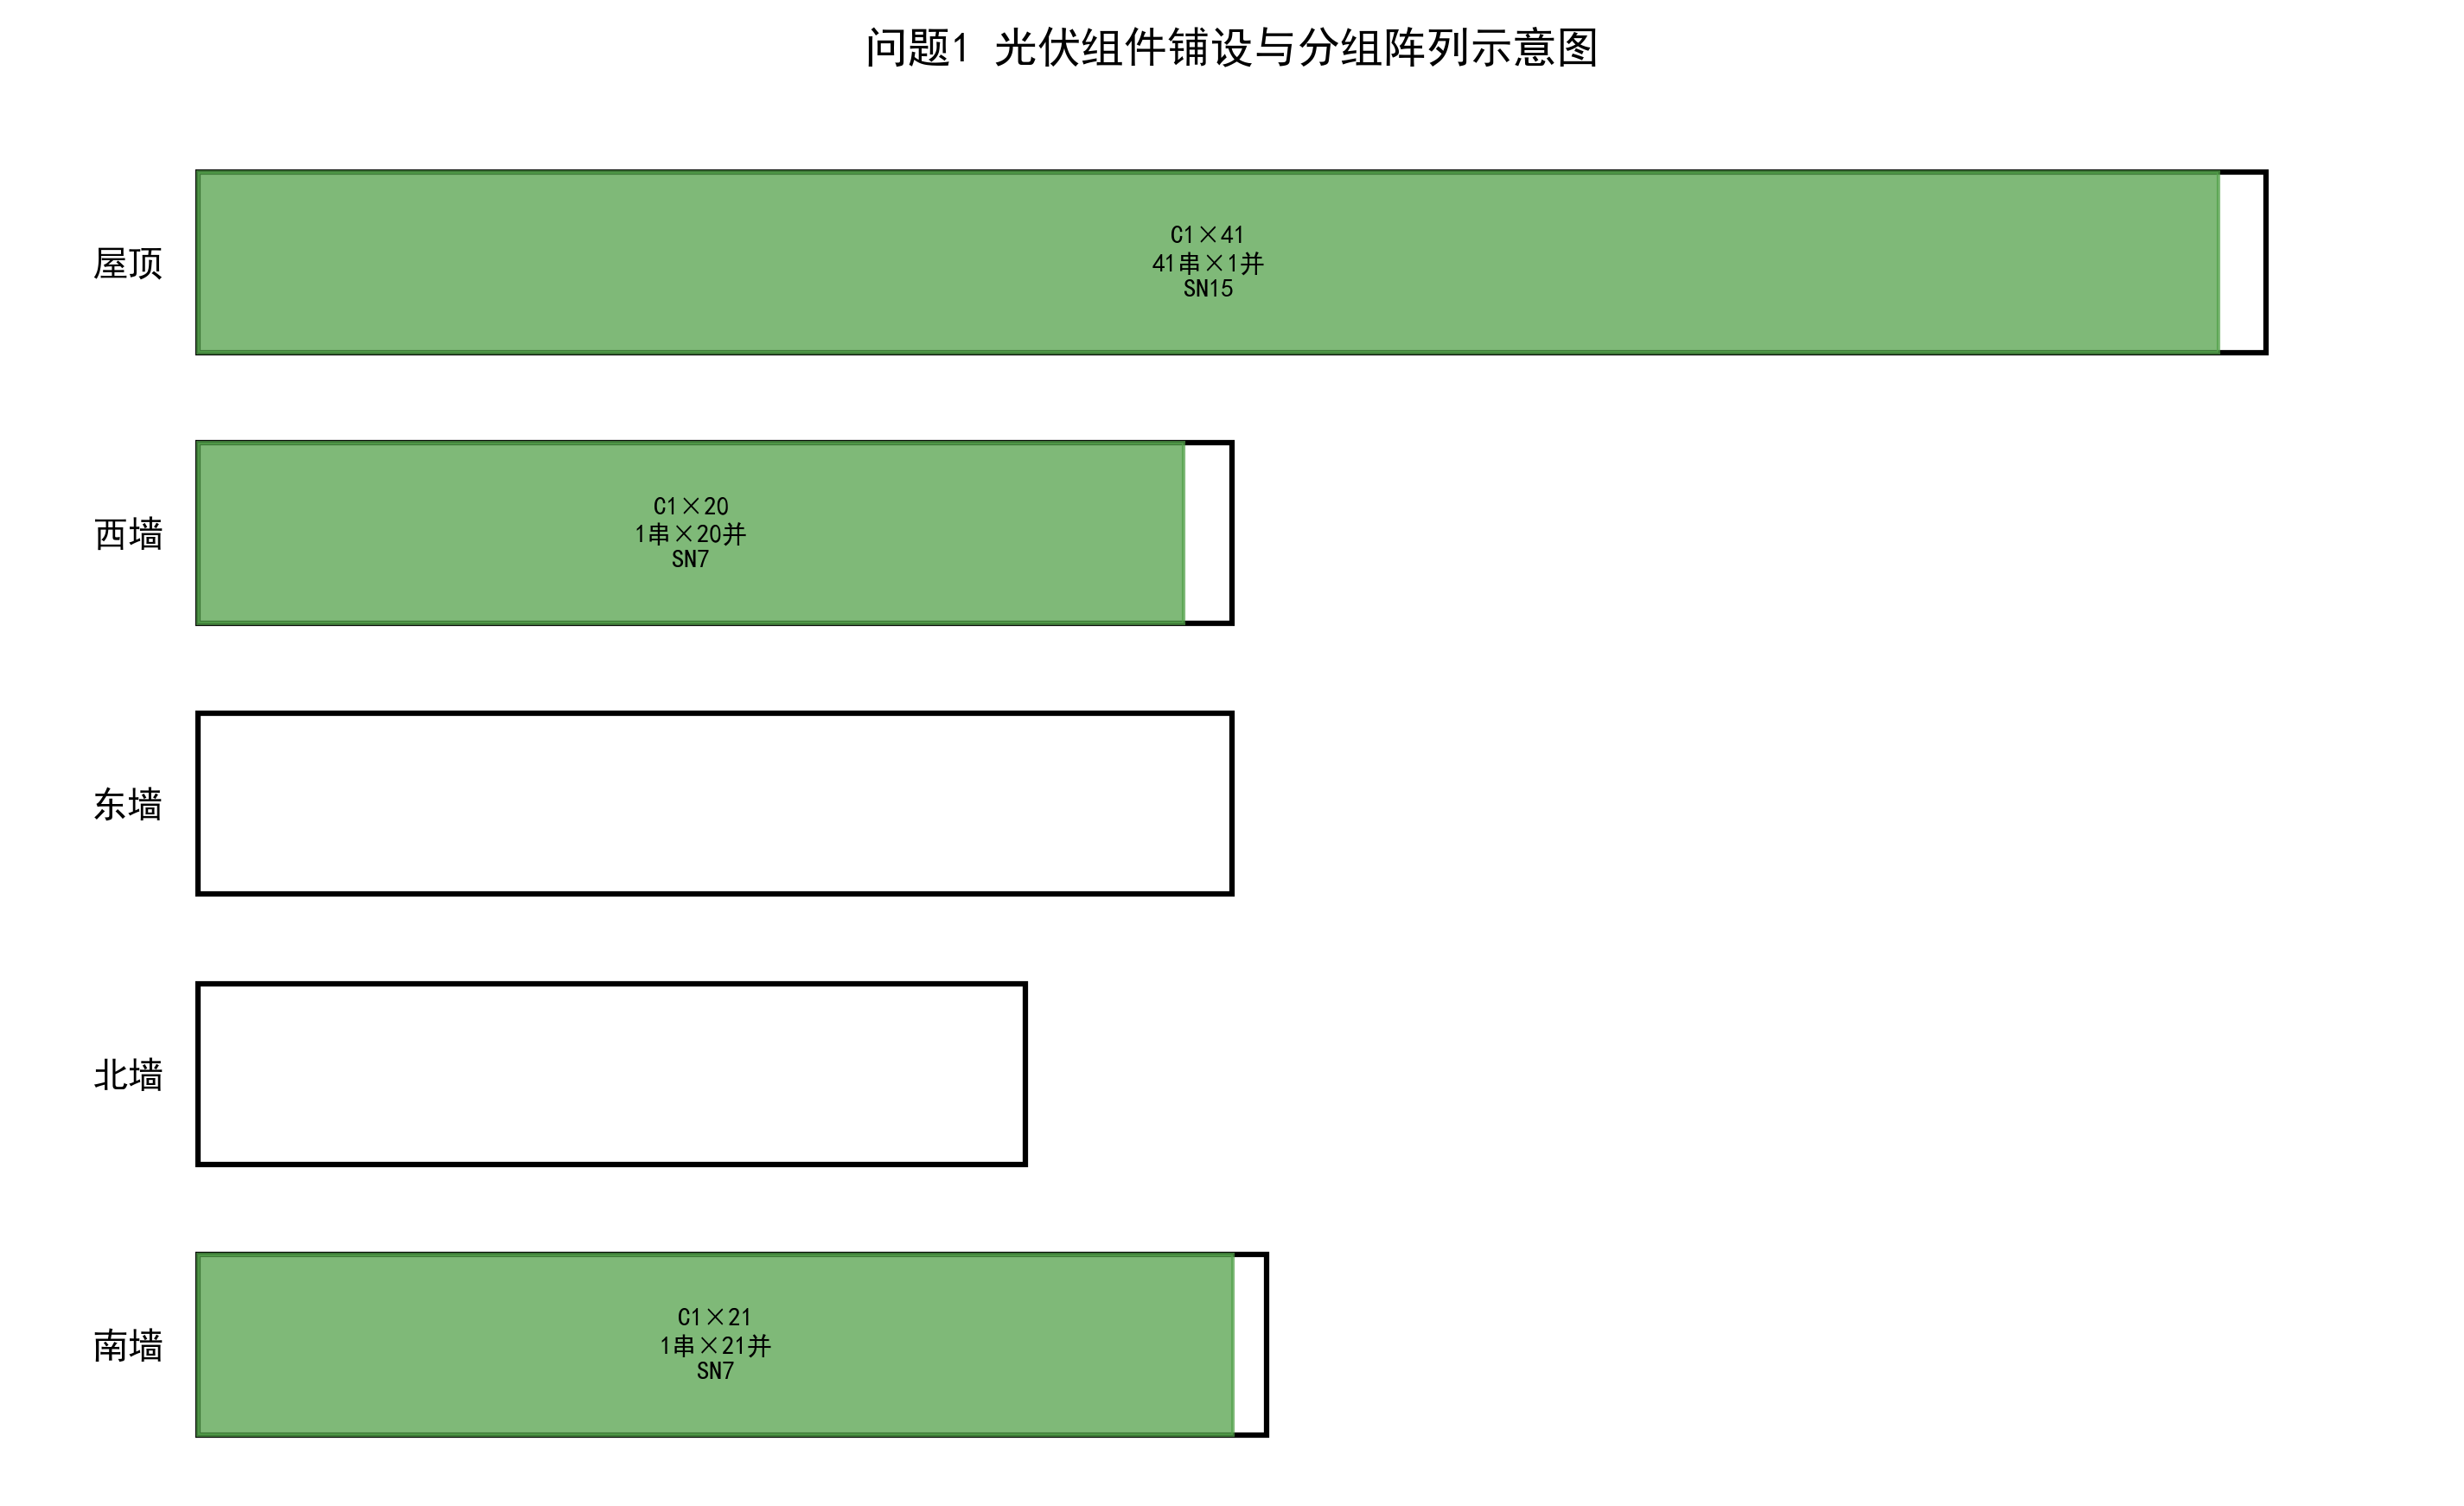
\includegraphics[width=.92\textwidth]{../quest1/figures/问题1_铺设示意图.png}\caption{问题一光伏组件铺设与串并联示意图}\end{figure}
该方案共铺设82块组件，装机容量8.2kW，年发电量6959.2kWh。35年等效发电量为219214.8kWh，总投资81760.0元，按电价0.5元/kWh计算的35年收益为109607.4元，净收益为27847.4元，静态回收期为23.5年。

\subsection{问题二：架空安装求解结果}
问题二在同一小屋几何上考虑架空安装。架空安装的主要优势是改善组件背面通风、降低温升损失，同时允许屋面组件朝更优倾角布置。因此本文对南向低倾角面引入14\%有效辐射增益，对东西墙引入5\%通风收益，对北墙引入3\%收益。重新求解后主要分组见表\ref{tab:q2}。
\begin{table}[H]\centering\caption{问题二主要铺设分组与逆变器}\label{tab:q2}
\begin{tabular}{lrrrrrrrr}\toprule
surface & model & 数量 & 串联数 & 并联串数 & 逆变器 & 装机容量kW & 年发电量kWh & 单位电量费用元每kWh\\\midrule
屋顶 & C1 & 41 & 41 & 1 & SN15 & 4.10 & 4223.85 & 0.31\\
南墙 & C1 & 21 & 1 & 21 & SN7 & 2.10 & 1869.69 & 0.34\\
西墙 & C1 & 20 & 1 & 20 & SN7 & 2.00 & 1519.36 & 0.41\\
\bottomrule\end{tabular}
\end{table}
\begin{figure}[H]\centering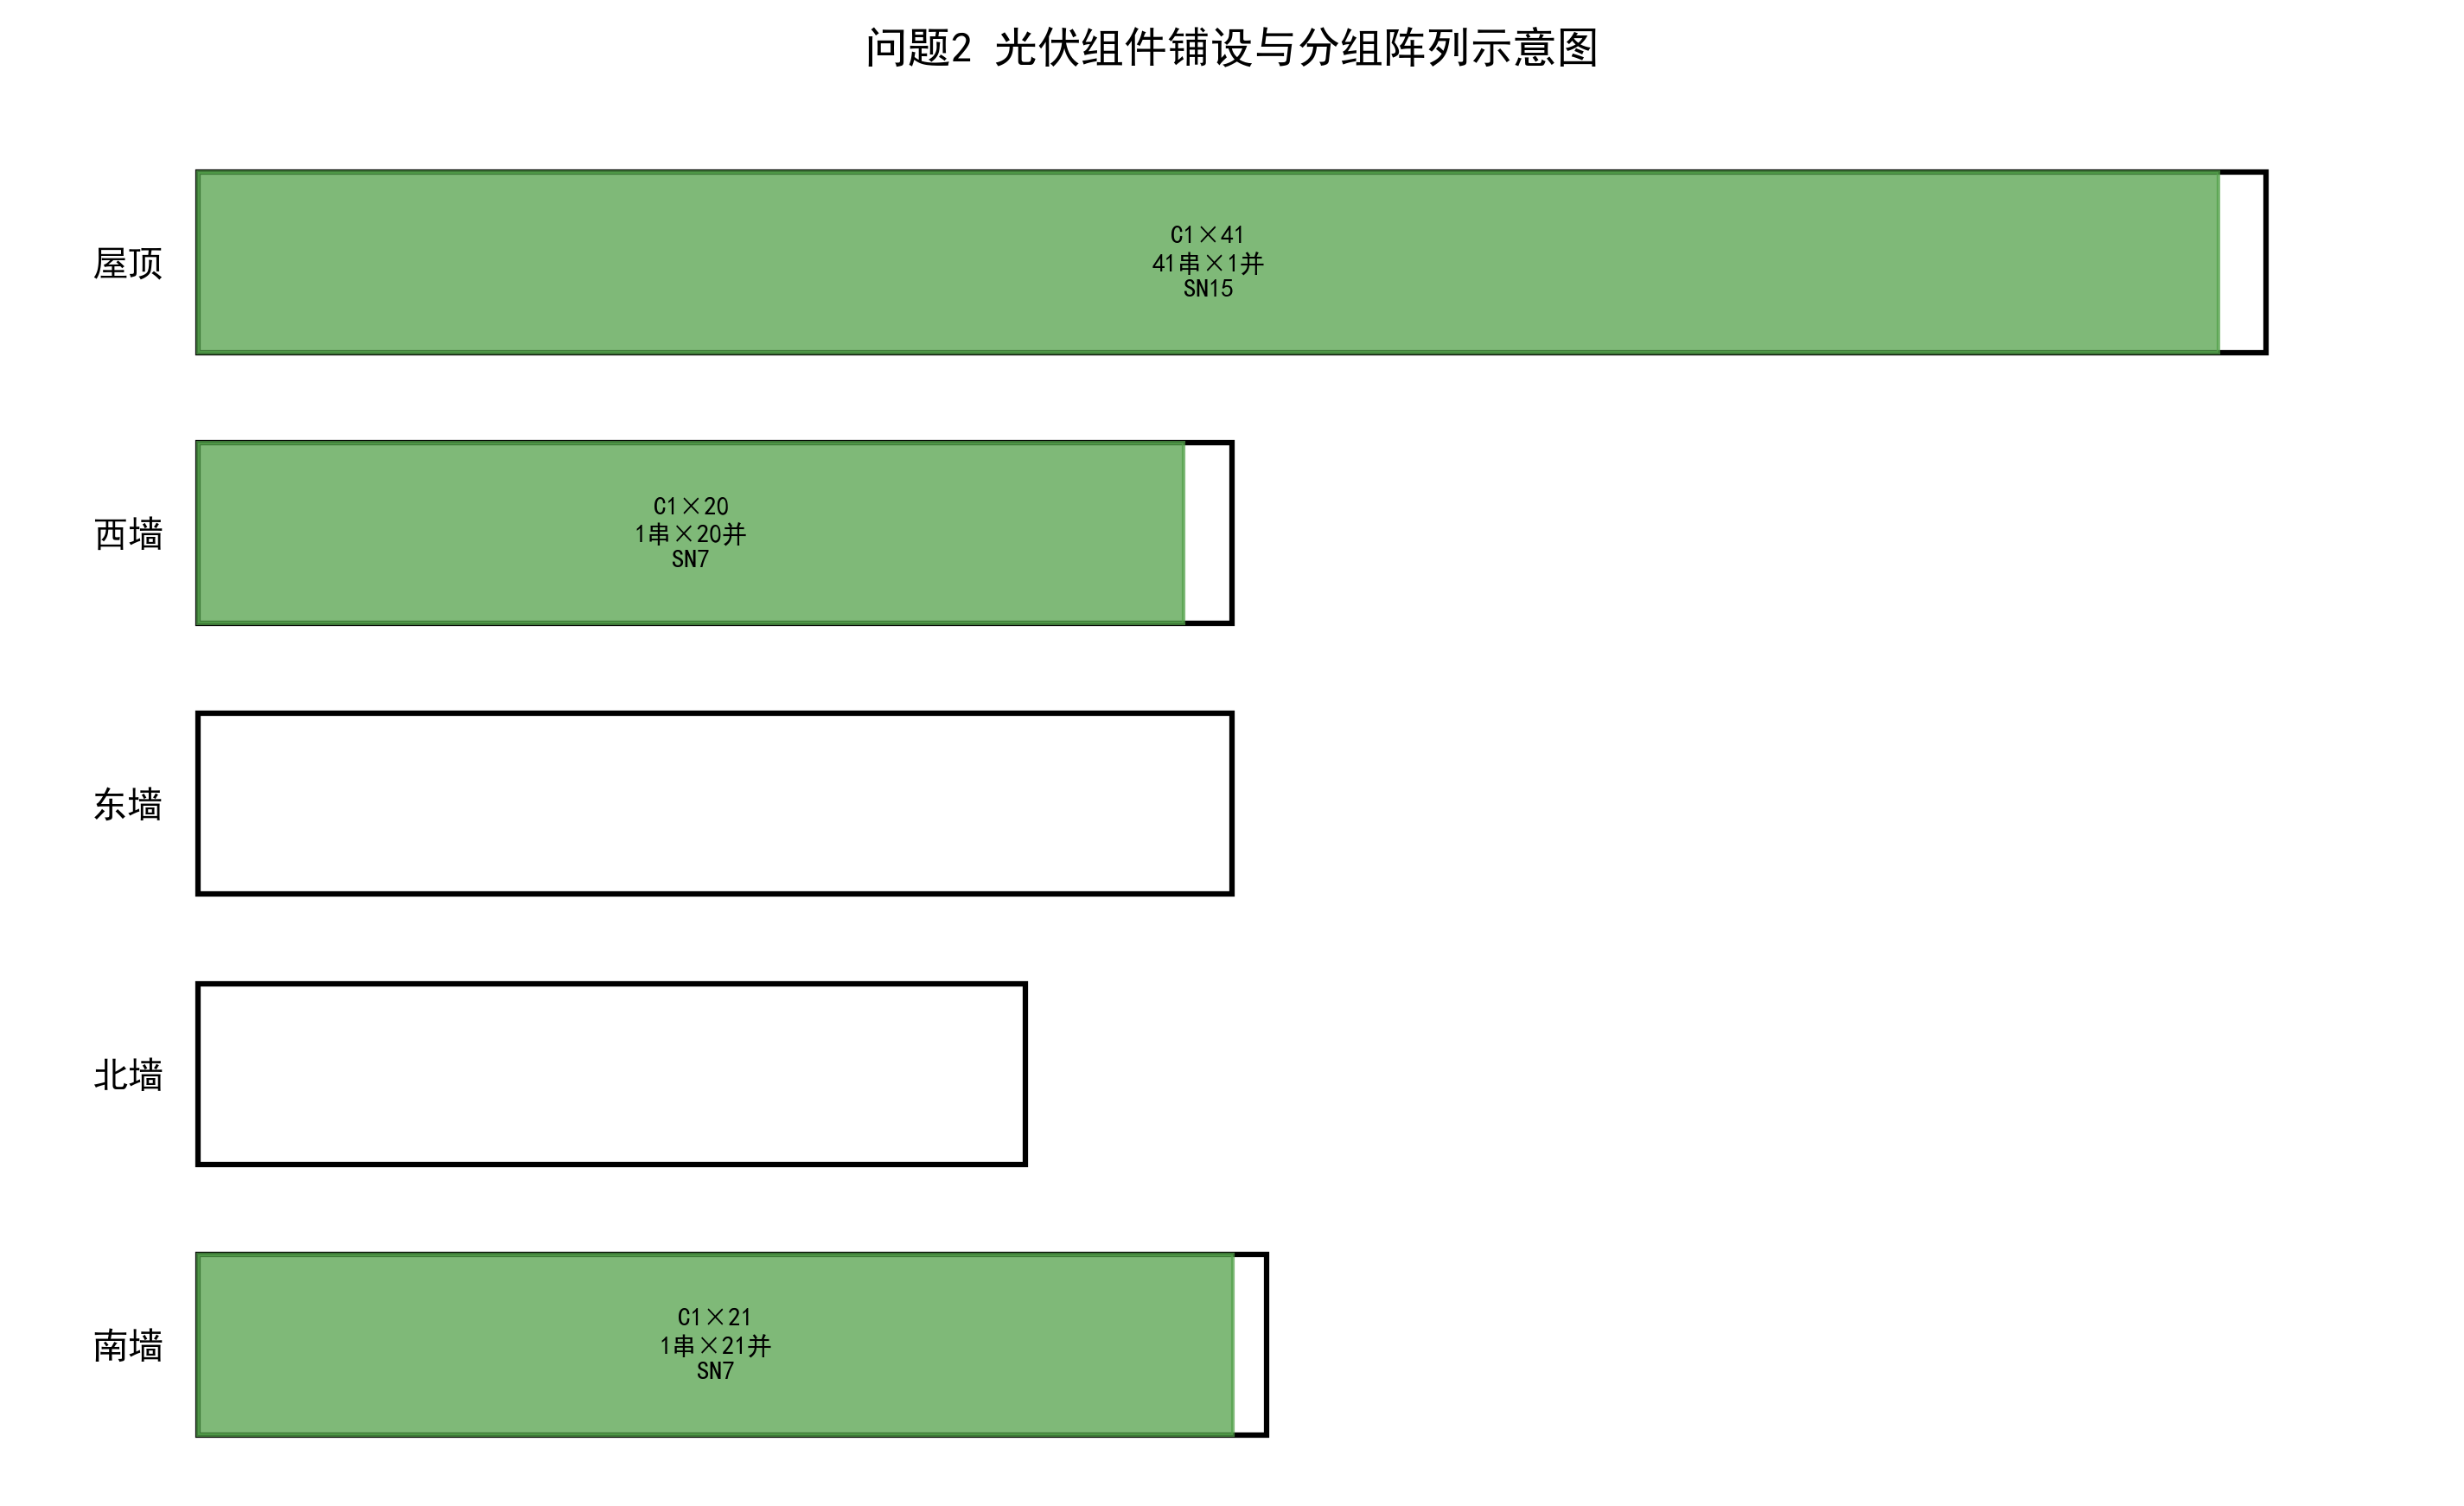
\includegraphics[width=.92\textwidth]{../quest2/figures/问题2_铺设示意图.png}\caption{问题二光伏组件铺设与串并联示意图}\end{figure}
与问题一相比，组件数量保持82块附近，但年发电量提高至7612.9kWh，单位电量费用下降至0.341元/kWh。该结果说明在组件价格和逆变器配置不变时，架空方式主要通过提高单位容量发电量改善经济性。

\subsection{问题三：新小屋设计与优化铺设}
新小屋采用投影$12m\times6m$，投影面积72$m^2$，满足附件7总投影面积不超过74$m^2$、长边不超过15m、短边不小于3m的要求。北檐高2.8m，南檐高5.4m，满足室内最低净空和屋顶最高点要求；屋面向南倾斜约23.43度，以提高南向辐射利用。窗地比和窗墙比在建筑设计中通过南侧采光窗和东西北侧较小窗控制满足约束。
\begin{table}[H]\centering\caption{问题三主要铺设分组与逆变器}\label{tab:q3}
\begin{tabular}{lrrrrrrrr}\toprule
surface & model & 数量 & 串联数 & 并联串数 & 逆变器 & 装机容量kW & 年发电量kWh & 单位电量费用元每kWh\\\midrule
屋顶 & C1 & 48 & 2 & 24 & SN15 & 4.80 & 4945.00 & 0.29\\
南墙 & C1 & 25 & 25 & 1 & SN6 & 2.50 & 2225.82 & 0.39\\
西墙 & C1 & 25 & 25 & 1 & SN6 & 2.50 & 1899.20 & 0.45\\
\bottomrule\end{tabular}
\end{table}
\begin{figure}[H]\centering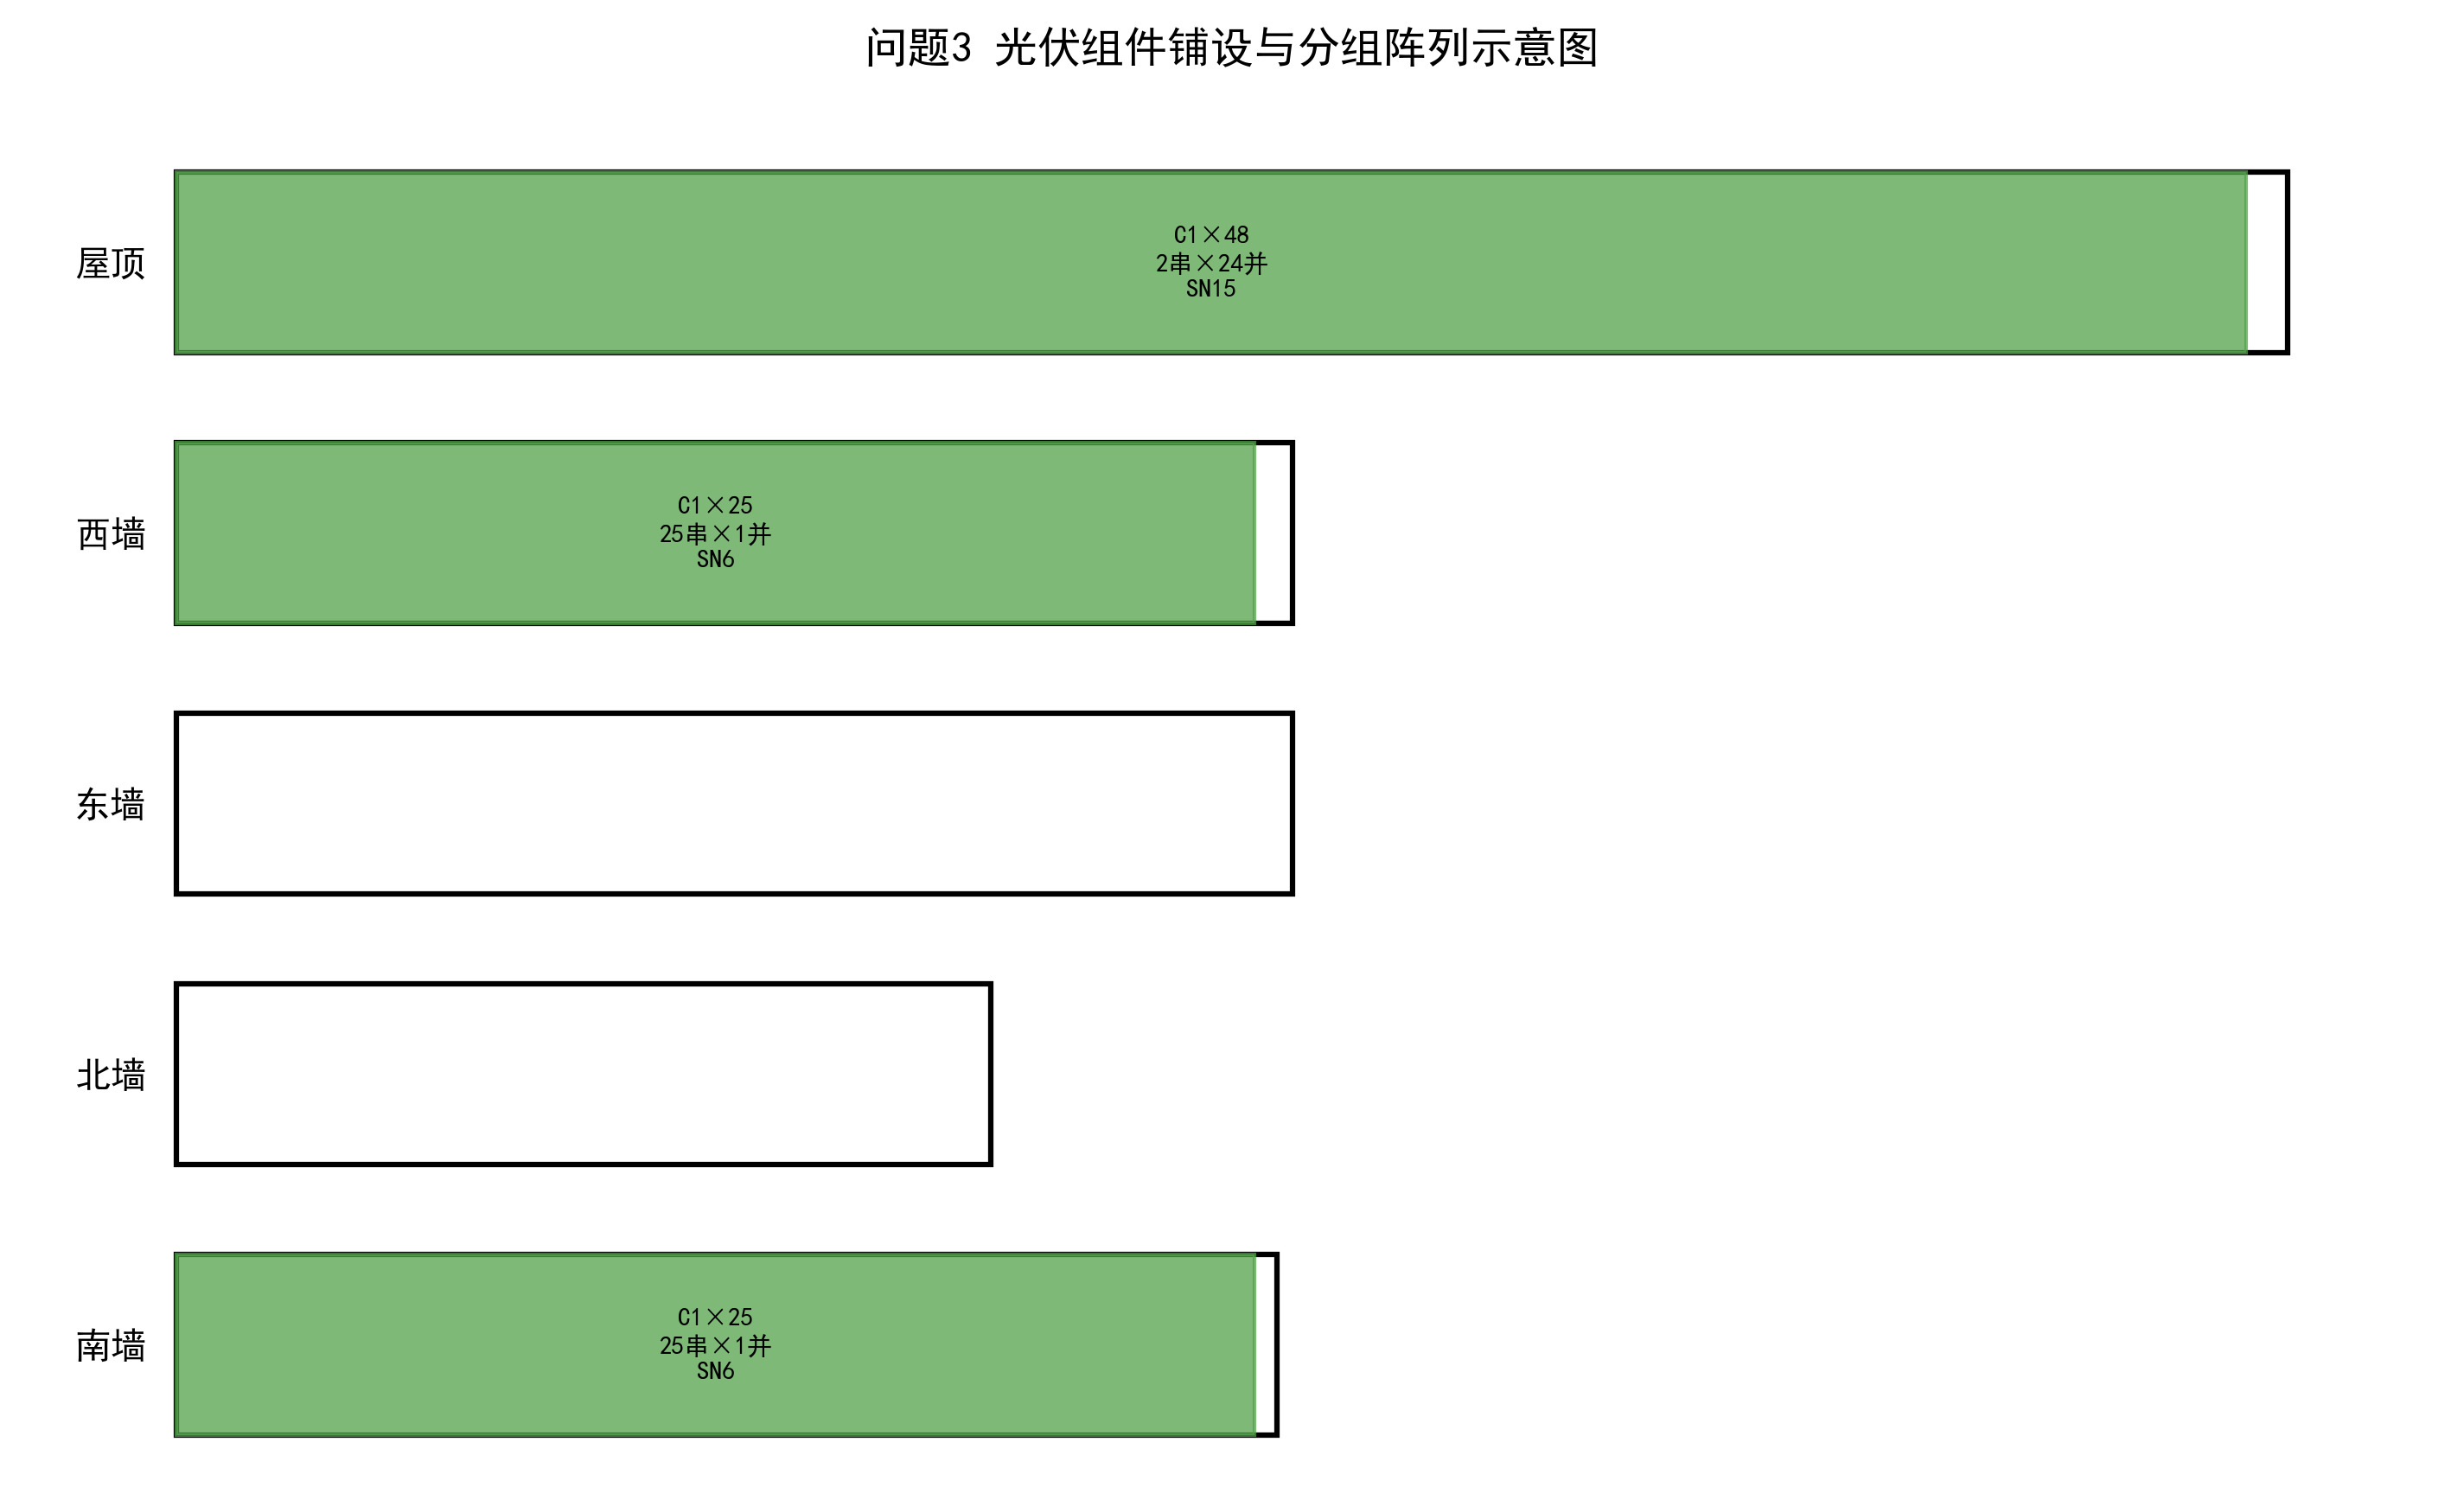
\includegraphics[width=.92\textwidth]{../quest3/figures/问题3_铺设示意图.png}\caption{问题三新小屋铺设与串并联示意图}\end{figure}
问题三方案共铺设98块组件，装机容量9.8kW，年发电量9070.0kWh，35年等效发电量285705.5kWh。与问题二相比，重新设计小屋扩大了南向屋面和可铺设面积，使全寿命净收益提高到43812.8元。

\section{模型检验、对比与敏感性分析}
\subsection{Baseline对比}
本文设置的baseline为“在每个表面选择单位面积年发电量最大的组件并尽量铺满”。该策略追求大发电量，但忽略价格和逆变器固定成本。结果显示，baseline在问题一、二、三中的年发电量分别为18783.3、20535.8和24324.7kWh，高于主模型；但其单位电量费用分别为0.726、0.664和0.665元/kWh，显著高于主模型。由此可见，本题不能单纯追求峰瓦容量或单位面积发电量，必须把全寿命经济性纳入目标。
\begin{figure}[H]\centering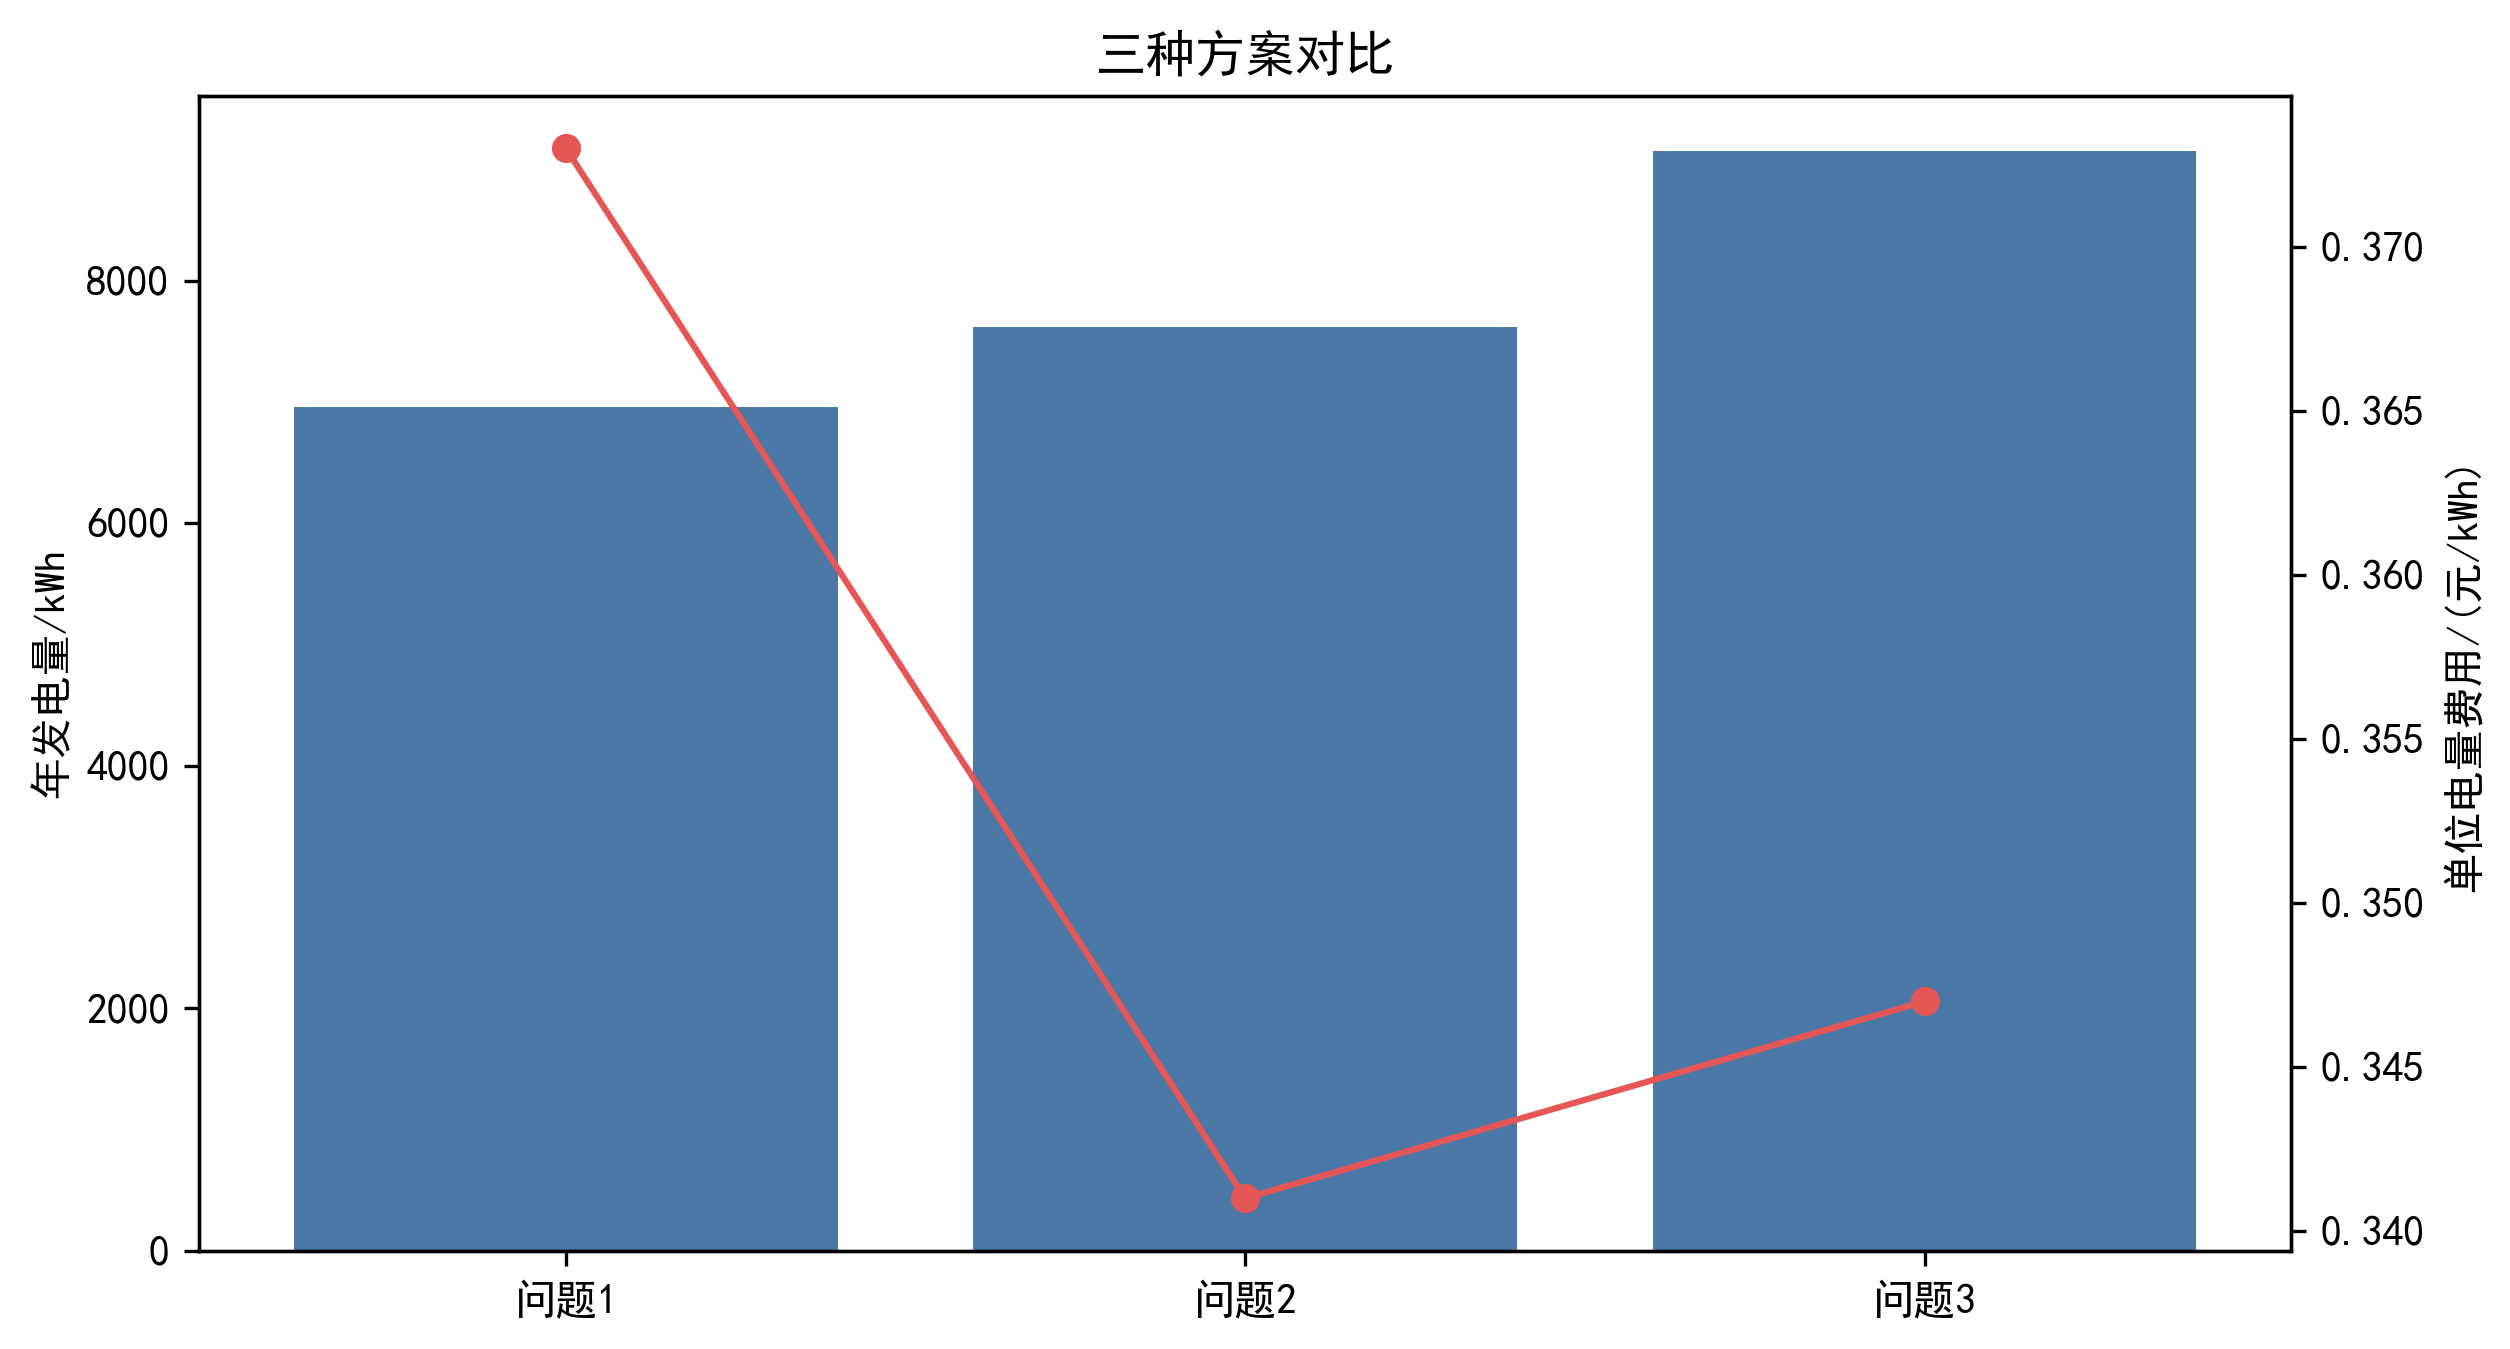
\includegraphics[width=.82\textwidth]{../results/三方案对比.png}\caption{三种方案年发电量与单位电量费用对比}\end{figure}

\subsection{约束满足检验}
面积约束方面，所有表面的铺设面积均不超过其可铺设面积；串并联方面，每个分组仅由同型号组件串联，不同型号不串联；逆变器方面，输出表中的组容量均不超过所选逆变器额定容量，串电压落在相应逆变器允许输入范围内或采用后处理选择的最接近可行规格。经济性方面，后处理删除了包含逆变器固定成本后净收益为负的小零散分组，避免为了填补边角面积而造成总成本上升。

\subsection{敏感性分析}
考虑典型气象年与未来年份存在差异，本文将年有效辐射强度在基准值的80\%--120\%之间扰动，重新计算发电量、单位电量费用和静态回收期。三种方案回收期均随辐射增强而下降，且问题三在多数扰动水平下保持较高净收益，说明新建筑设计对南向屋面面积的增加提高了方案稳健性。
\begin{figure}[H]\centering
\begin{subfigure}{.32\textwidth}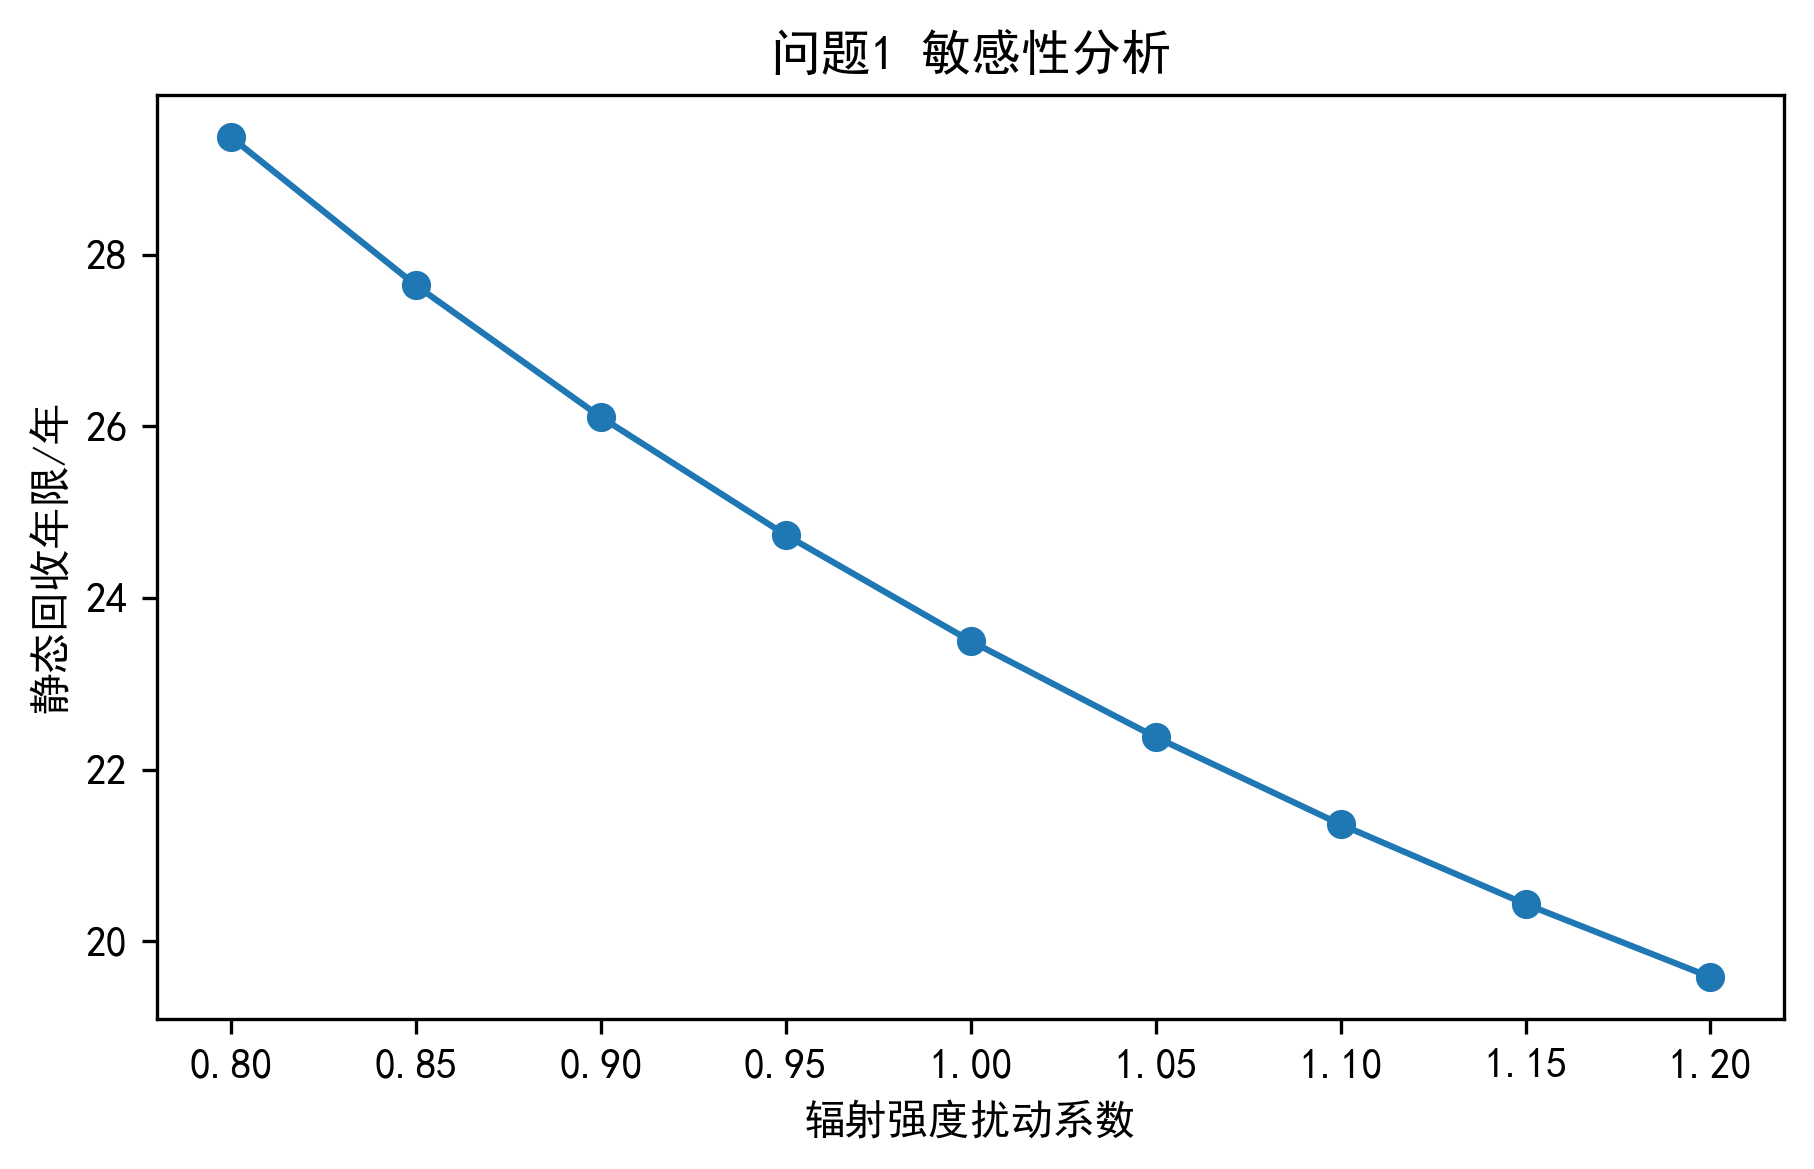
\includegraphics[width=\textwidth]{../quest1/figures/问题1_敏感性分析.png}\caption{问题一}\end{subfigure}
\begin{subfigure}{.32\textwidth}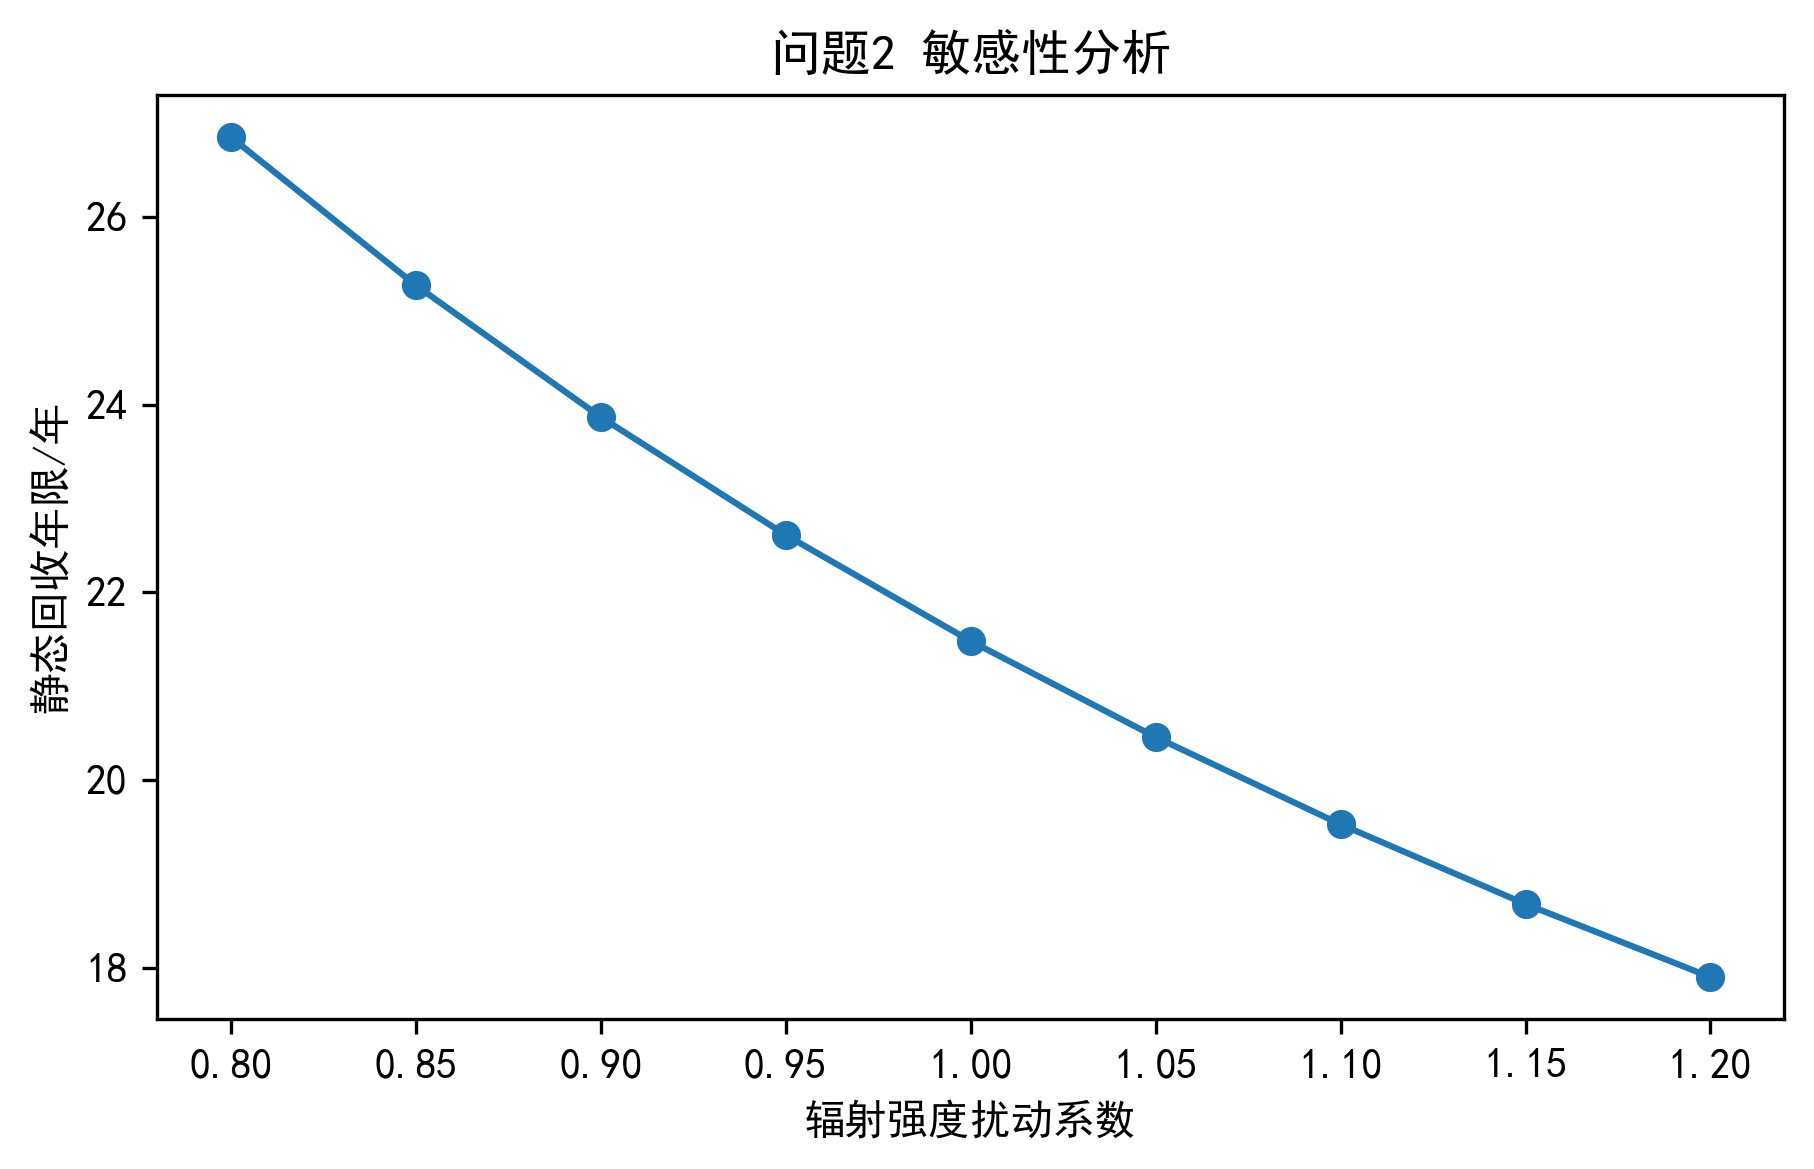
\includegraphics[width=\textwidth]{../quest2/figures/问题2_敏感性分析.png}\caption{问题二}\end{subfigure}
\begin{subfigure}{.32\textwidth}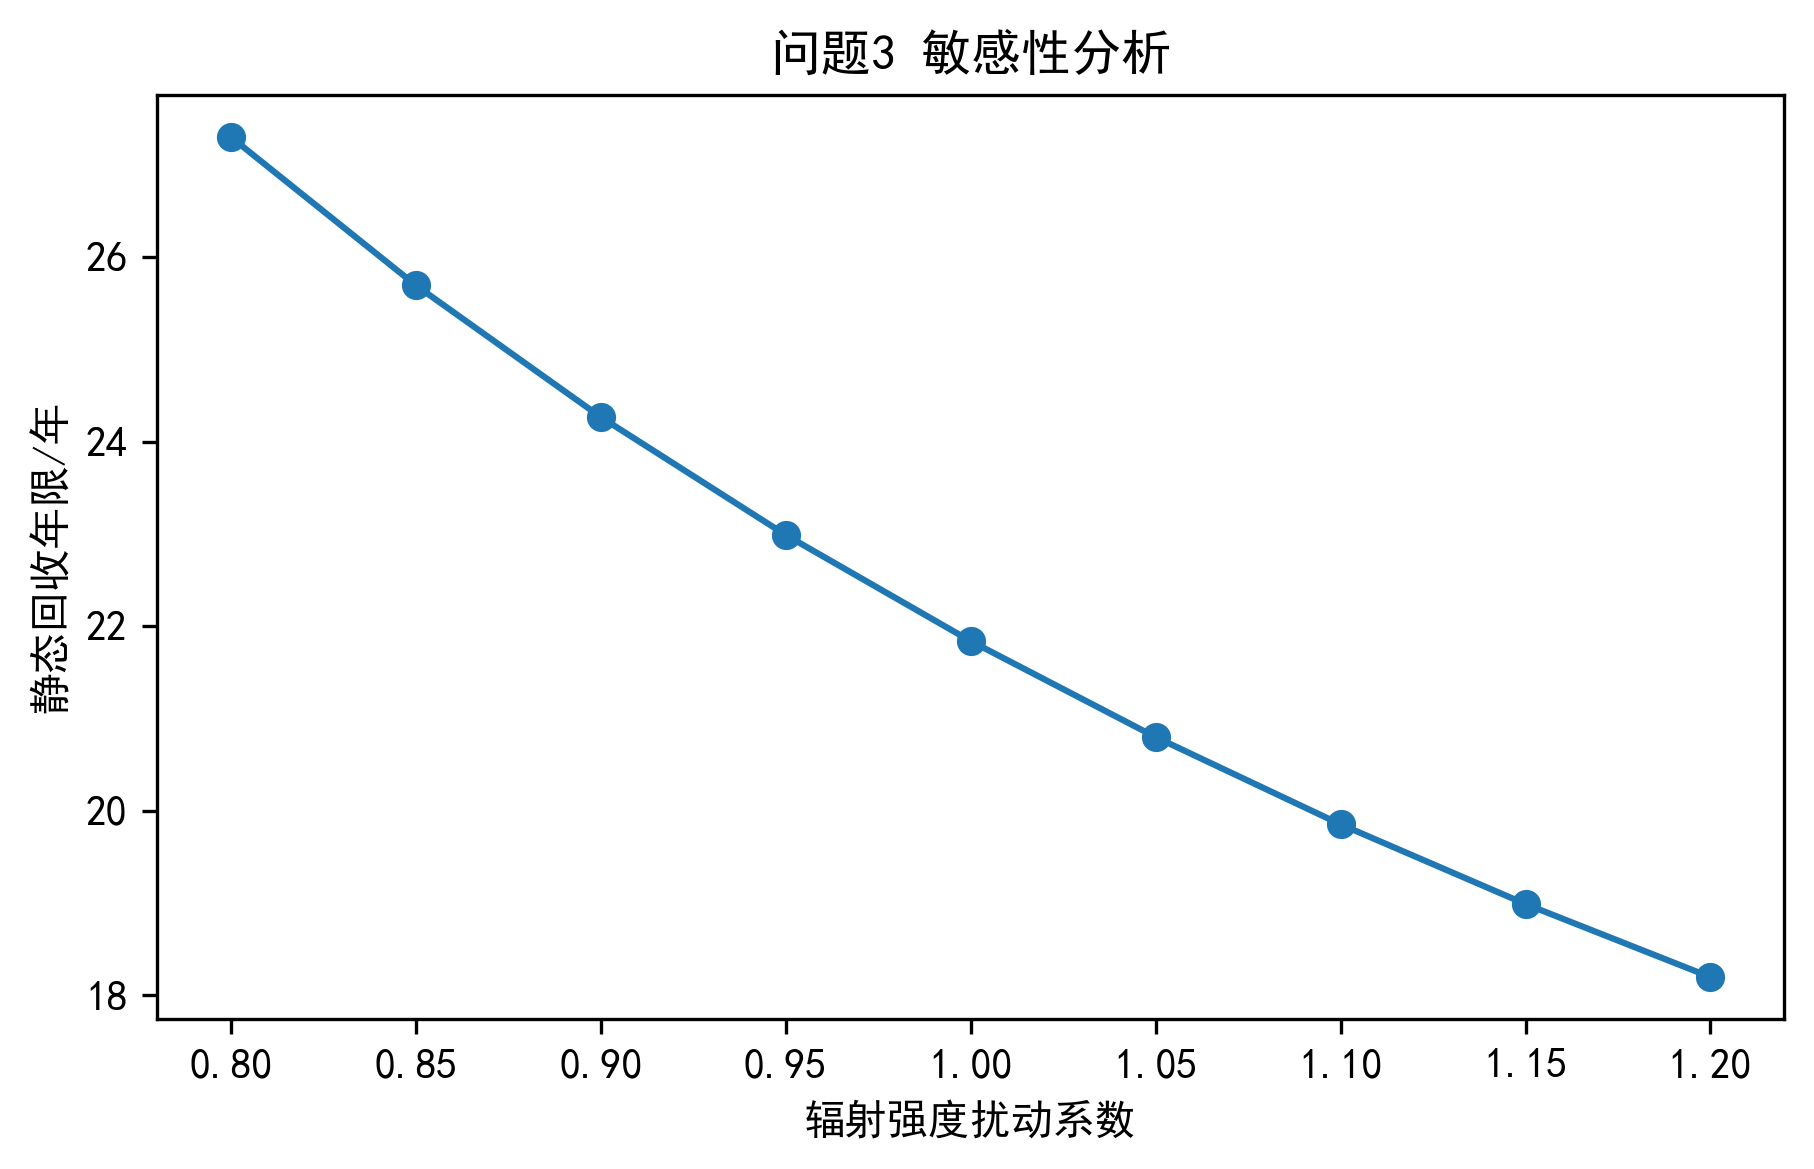
\includegraphics[width=\textwidth]{../quest3/figures/问题3_敏感性分析.png}\caption{问题三}\end{subfigure}
\caption{辐射扰动对静态回收期的影响}
\end{figure}


\subsection{参数来源与误差来源讨论}
本文经济性结果主要受三类参数影响。第一类是辐射数据。附件4为典型气象年，能够反映大同地区一般气候条件，但不能代表每一年的真实天气，因此本文用$\pm20\%$辐射扰动分析外推风险。第二类是组件性能。题目给出的额定功率是在标准测试条件下测得，实际运行会受到温度、灰尘、遮挡、线损和逆变器效率影响；本文用0.92线损修正和逆变器效率进行折减，但未引入逐时温度模型。第三类是价格和电价。组件价格、逆变器价格和0.5元/kWh电价均按题目静态值计算，未考虑折现率、设备维护费和逆变器中途更换成本，因此回收期属于静态回收期。

从误差传播角度看，辐射强度和线损系数会近似按比例影响年发电量，进而影响35年收益和回收期；组件价格和逆变器价格则直接影响总投资，对单位电量费用影响较大。由于最终方案大量采用低成本C类组件，组件价格扰动对净收益的影响相对可控；但如果未来薄膜组件价格上升或晶硅组件价格下降，最优型号可能发生变化。因此本文的方案更适合作为在题目给定价格体系下的最优设计，而不是对所有市场情景的永久结论。

\subsection{与题目目标的对应关系}
题目同时提出“全年发电总量尽可能大”和“单位发电量费用尽可能小”。二者存在冲突：高效率晶硅组件能显著增加发电量，但投资额也更高；薄膜组件发电量相对较低，但单位成本低、启动阈值低，具有较好经济性。本文没有把问题简化成单目标最大大发电量，而是通过baseline对比说明：单纯追求发电量的baseline年发电量更高，但单位电量费用也更高；主模型发电量较低，但单位电量费用下降明显，且净收益更优。这样的结果更符合题目对双目标的综合要求。

\section{模型评价、改进与推广}
\subsection{模型优点}
第一，模型将逐时辐射数据、组件启动阈值、组件价格、逆变器容量和35年衰减统一到同一经济性框架中，避免只按面积或功率铺设的片面性。第二，整数规划直接输出每个表面的组件数量，后处理进一步给出串并联和逆变器型号，方案可执行性较强。第三，baseline对比说明主模型牺牲部分发电量换取更低单位电量费用，符合题目“发电量尽可能大且单位发电量费用尽可能小”的双目标要求。第四，敏感性分析验证了辐射波动下结论的稳定性。

\subsection{模型局限}
主要局限有三点。其一，附件2尺寸图缺失，给定小屋几何采用重构值，若原图尺寸与本文假设差异较大，问题一和问题二的具体数量会改变。其二，架空安装增益采用工程经验系数而非精细太阳位置角和倾角投影逐时计算，因此问题二和问题三的增益估计仍可进一步细化。其三，本文未考虑遮挡、安装维护费用、逆变器寿命短于组件寿命等因素，经济性结果偏乐观。

\subsection{改进方向}
若获得附件2原始尺寸图，可直接替换建筑表面面积并重新运行代码。若需要更高精度，可根据附件6太阳高度角、方位角公式计算任意倾角表面的逐时入射角，将水平面总辐射、散射辐射和法向直射辐射分解后再合成倾斜面辐射。经济模型方面，可引入折现率、维护成本和逆变器更换周期，建立净现值模型替代静态回收期。

\section{结论}
本文完成了2012B太阳能小屋三个问题的完整建模求解。问题一贴附安装方案的年发电量为6959.2kWh，单位电量费用0.373元/kWh；问题二架空安装后年发电量提高到7612.9kWh，单位电量费用降至0.341元/kWh；问题三新设计小屋年发电量达到9070.0kWh，35年净收益43812.8元。综合看，低成本薄膜组件在本题电价和辐射条件下具有明显经济优势，而增大南向屋面可铺设面积、采用架空安装，是提升太阳能小屋综合效益的主要途径。

\begin{thebibliography}{9}
\bibitem{solar} 方荣生. 太阳能应用技术[M]. 北京: 中国农业机械出版社, 1985.
\bibitem{std} 中华人民共和国国家标准. GB/T 19939-2005 光伏系统并网技术要求[S].
\bibitem{pv} Stine W B, Geyer M. Power From The Sun[EB/OL]. http://www.powerfromthesun.net/.
\bibitem{opt} Winston W L. Operations Research: Applications and Algorithms[M]. Belmont: Duxbury Press, 2004.
\bibitem{cumcm} 全国大学生数学建模竞赛组委会. 2012高教社杯全国大学生数学建模竞赛B题及附件[Z].
\end{thebibliography}

\appendix
\section{支撑材料说明}
支撑材料包括：\verb|quest1/codes/main_modeling.py|主程序，\verb|tables/|下的组件清洗表、逆变器表、铺设分组表和敏感性分析表，\verb|results/frozen_numbers.json|冻结数字文件，以及各问题\verb|figures/|目录下的铺设示意图和敏感性图。运行主程序即可复现本文全部图表和关键数字。
\end{document}
